\chapter{trait与泛型}\label{ch11}

\emph{[A] computer scientist tends to be able to deal with nonuniform structures—case 1, case 2, case 3—while a mathematician will tend to want one unifying axiom that governs an entire system.}

\begin{flushright}
    ——Donald Knuth
\end{flushright}

编程界中最伟大的发现之一就是可以编写处理多种不同类型的代码,\emph{即使是还没有定义出来的类型也可以}。这里有两个例子:
\begin{itemize}
    \item \texttt{Vec<T>}是泛型的:你可以创建一个任意类型的vector,包括你自己定义的类型,即使\texttt{Vec}的作者完全不知道这个类型。
    \item 很多类型都有\texttt{.write()}方法,包括\texttt{File}和\texttt{TcpStream}。你的代码可以通过引用获取一个writer(任意的writer),并向它写入数据。你的代码不需要关心那个writer到底是什么类型。然后,如果有人添加了一个新的writer类型,你的代码将会自动支持它。
\end{itemize}

当然,这并不是什么新鲜的功能。它被称为\emph{多态(polymorphism)},是20世纪70年代很热门的新的编程语言技术。但现在它已经非常普遍了。Rust使用两个相关的特性来支持多态:trait和泛型。很多程序员可能已经很熟悉这两个概念了,但Rust采用了一种受Haskell的typeclass启发的新方法。

\emph{trait}是Rust中的接口或抽象基类。首先,它们看起来很像Java或C\#中的接口。用于写入字节的trait叫做\texttt{std::io::Write},它在标准库中的定义看起来像这样:
\begin{minted}{Rust}
    trait Write {
        fn write(&mut self, buf: &[u8]) -> Result<usize>;
        fn flush(&mut self) -> Result<()>;

        fn write_all(&mut self, buf: &[u8]) -> Result<()> { ... }
        ...
    }
\end{minted}

这个trait提供了几个方法,我们只展示了前三个。

标准类型\texttt{File}和\texttt{TcpStream}都实现了\texttt{std::io::Write}。\texttt{Vec<u8>}也是。这三个类型都提供\texttt{.write()}、\texttt{.flush()}等方法。使用writer的代码不需要关心它的类型,像这样:
\begin{minted}{Rust}
    use std::io::Write;

    fn say_hello(out: &mut dyn Write) -> std::io::Result<()> {
        out.write_all(b"hello world\n")?;
        out.flush()
    }
\end{minted}

\texttt{out}的类型是\texttt{\&mut dyn Write},意思是“任何实现了。\texttt{Write} trait的值的可变引用”。我们可以把任何这样的值的可变引用传递给\texttt{say\_hello}:
\begin{minted}{Rust}
    use std::fs::File;
    let mut local_file = File::create("hello.txt")?;
    say_hello(&mut local_file)?;    // 可以工作

    let mut bytes = vec![];
    say_hello(&mut bytes)?;         // 也可以工作
    assert_eq!(bytes, b"hello world\n");
\end{minted}

这一章首先展示trait怎么使用、怎么工作、怎么定义自己的trait。但trait的用途比我们目前提到的更多。我们将使用它们给现有类型添加扩展的方法,甚至像\texttt{str}和\texttt{bool}这种内建类型也可以。我们将会解释为什么给一个类型添加trait不会消耗多余的内存,以及如何在没有虚方法开销的情况下使用trait。我们将看到一些Rust提供的用于操作符重载和其他特性的语言内建的trait。我们还将介绍\texttt{Self}类型、关联函数、关联类型。Rust从Haskell中提取了这三个特性,它们可以优雅地解决其他语言中需要通过变通的方法或者hack才能解决的问题。 

\emph{泛型}是Rust中另一种形式的多态。类似于C++的模板,一个泛型函数或类型可以用于多种不同的类型:
\begin{minted}{Rust}
    /// 给定两个值,找出较小的那个
    fn min<T: Ord>(value1: T, value2: T) -> T {
        if value1 <= value2 {
            value1
        } else {
            value2
        }
    }
\end{minted}

这个函数中的\texttt{<T: Ord>}意味着\texttt{min}可以用于任何实现了\texttt{Ord} trait的类型\texttt{T}——也就是,任何有序的类型。这样的一个要求被称为\emph{约束(bound)},因为它列举出了类型\texttt{T}需要满足的限制。编译器会为你实际使用的每一个类型\texttt{T}生成自定义的机器代码。

泛型和trait紧密相关:泛型函数在约束中使用trait来表明它可以用于哪些类型的参数。所以我们还会讨论\texttt{\&mut dyn Write}和\texttt{<T: Write>}有哪些相似和不同之处,以及如何在这种两种使用trait的方式中选择。

\section{使用trait}

一个trait就是一个给定的类型可能支持也可能不支持的特性。通常,一个trait代表一种能力:一个类型可以做的事情。
\begin{itemize}
    \item 一个实现了\texttt{std::io::Write}的值可以写入字节。
    \item 一个实现了\texttt{std::iter::Iterator}的值可以产生值的序列。
    \item 一个实现了\texttt{std::clone::Clone}的值可以产生自身在内存中的克隆。
    \item 一个实现了\texttt{std::fmt::Debug}可以使用\texttt{println!()}的\texttt{\{:?\}}格式说明符进行打印。
\end{itemize}

那4个trait都是Rust标准库的一部分,有很多标准类型都实现了它们。例如:
\begin{itemize}
    \item \texttt{std::fs::File}实现了\texttt{Write} trait,它把字节写入到本地文件。\texttt{std::net::TcpStream}写入到网络连接。\texttt{Vec<u8>}也实现了\texttt{Write}。在字节vector上调用\texttt{.write()}会往尾部添加数据。
    \item \texttt{Range<i32>}(\texttt{0..10}的类型)实现了\texttt{Iterator} trait,一些和切片、哈希表等相关联的迭代器类型也实现了这个trait。
    \item 大多数标准库类型实现了\texttt{Clone}。一些例外主要是像\texttt{TcpStream}这样的不仅仅表示内存中的数据的类型。
    \item 大多数标准库类型支持\texttt{Debug}。
\end{itemize}

有关trait方法有一个不寻常的规则:trait自身必须在作用域里。否则,所有它的方法都会被隐藏:
\begin{minted}{Rust}
    let mut buf: Vec<u8> = vec![];
    buf.write_all(b"hello")?;   // 错误:没有叫`write_all`的方法
\end{minted}

这种情况下,编译器会打印出友好的错误消息建议你添加\texttt{std::io::Write},然后确实能修复这个问题:
\begin{minted}{Rust}
    use std::io::Write;

    let mut buf: Vec<u8> = vec![];
    buf.write_all(b"hello")?;   // ok
\end{minted}

Rust会有这个规则是因为,正如我们稍后会在本章中看到的,你可以使用trait来给任意类型添加新的方法——即使是标准库的类型例如\texttt{u32}和\texttt{str}。第三方的crate也可以做同样的事情。显然,这会导致名称冲突!但因为Rust让你自己导入你需要使用的trait,所以crate可以轻松地利用这种强大的功能。要想导致冲突,你需要导入两个trait,这两个trait要给同一个类型添加相同名称的方法。这在实践中是很少见的。(如果你确实陷入了冲突中,你可以使用本章稍后会介绍的\nameref{fullymethod}来指明你想要使用哪一个。)

\texttt{Clone}和\texttt{Iterator}的方法不需要特殊的导入是因为它们默认总是在作用域里,它们是标准prelude的一部分:Rust会自动导入每个模块中的名称。事实上,prelude就是一个精心挑选的trait的集合。我们将在\hyperref[ch13]{第13章}中介绍更多有关它们的内容。

C++和C\#程序员可能已经注意到了trait方法很像虚方法。然而,类似上面的函数调用速度很快,与任何其他方法调用一样快。简单来说,这里面并没有多态性。显然\texttt{buf}是一个vector,不是一个文件或者网络连接,所以编译器可以简单地生成一个\texttt{Vec<u8>::write()}的调用。它甚至可以内联这个方法。(C++和C\#通常也会这样,尽管子类化的可能性有时会排除这一点。)只有通过\texttt{\&mut dyn Write}的调用才会有动态分发的开销,这种调用也被称为虚方法调用,类型里的\texttt{dyn}关键字暗示了这一点。\texttt{dyn Write}被称为\emph{trait对象(trait object)};我们将会在接下来的小节中看到trait对象的技术细节,以及它们与泛型函数的比较。

\subsection{trait对象}\label{traitobject}
在Rust中有两种使用trait来编写多态代码的方式:trait对象和泛型。我们将会首先介绍trait对象,在下一节中介绍泛型。

Rust不允许\texttt{dyn Write}类型的变量:
\begin{minted}{Rust}
    use std::io::Write;

    let mut buf: Vec<u8> = vec![];
    let writer: dyn Write = buf; // 错误:`Write`并没有固定的大小
\end{minted}

一个变量的大小必须在编译期时已知,然而实现了\texttt{Write}的类型可以是任何大小。

如果你来自C\#或者Java的话可能会感觉很惊讶,但原因其实很简单。在Java中,一个\texttt{OutputStream}(Java中类似\texttt{std::io::Write}的标准接口)类型的变量是一个任何实现了\texttt{OutputStream}的对象的引用。它是一个引用的事实不言而喻,C\#以及其他大多数语言中的接口也是一样。

我们在Rust中想要的也是一样的,但是在Rust中引用是显式的:
\begin{minted}{Rust}
    let mut buf: Vec<u8> = vec![];
    let writer: &mut dyn Write = &mut buf;  // ok
\end{minted}

一个trait类型的引用,例如\texttt{writer},被称为一个\emph{trait对象}。和其他引用一样,一个trait对象指向某个值、它有生命周期、它可以是可变的或者是共享的。

让一个trait对象与众不同的是Rust在编译期通常不知道被引用值的类型是什么。因此一个trait对象包括一点额外的有关被引用值的类型信息。类型信息被严格限制为只有Rust自己可以在幕后使用:当你调用\texttt{writer.write(data)}时,Rust需要这个类型信息来依据\texttt{*writer}的类型动态调用正确的\texttt{write}方法。你不能直接查询类型信息,Rust也不支持将trait对象\texttt{\&mut dyn Write}向下转换回精确的类型例如\texttt{Vec<u8>}。

\subsubsection{trait对象的布局}
在内存中,一个trait对象是一个胖指针,由指向值的指针加上一个指向表示该值类型的表的指针组成。因此每一个trait对象要占两个机器字,如\hyperref[f11-1]{图11-1}所示。

\begin{figure}[htbp]
    \centering
    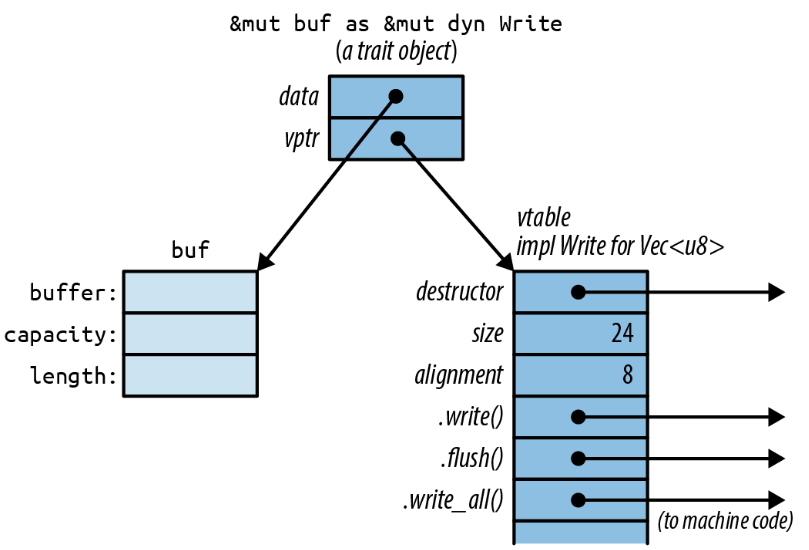
\includegraphics[width=0.9\textwidth]{../img/f11-1.png}
    \caption{内存中的trait对象}
    \label{f11-1}
\end{figure}

C++也有这种运行时的类型信息。它被称为\emph{虚表}或者\emph{vtable}。在Rust中和在C++中一样,vtable只会在编译期生成一次,然后被所有相同类型的对象共享。\hyperref[f11-1]{图11-1}中较深颜色的阴影显示的内容,包括vtable,都是Rust的私有实现。这些字段和数据结构你不能直接访问。当你调用trait对象的方法时语言本身会自动使用vtable来决定要调用哪个实现。

熟练的C++程序员可能会注意到Rust和C++采取的内存策略有些不同。在C++中,虚表指针或者称为\emph{vptr}被存储为结构体的一部分,而Rust使用胖指针来代替。结构体本身不包含任何自身字段之外的东西。这样,一个结构体可以实现一大堆trait而不需要包含一大堆vptr。即使像\texttt{i32}这样的大小还不足以容纳一个vptr的类型,也可以实现trait。

当需要时Rust会自动把普通引用转换为trait对象。这就是为什么我们能在这个例子中直接把\texttt{\&mut local\_file}传递给\texttt{say\_hello}:
\begin{minted}{Rust}
    let mut local_file = File::create("hello.txt")?;
    say_hello(&mut local_file)?;
\end{minted}

\texttt{\&mut local\_file}的类型是\texttt{\&mut File},而\texttt{say\_hello}的参数类型是\texttt{\&mut dyn Write}。因为\texttt{File}是一种writer,所以Rust允许这种普通引用到trait对象的转换。

同样的,Rust也乐于把\texttt{Box<File>}转换成\texttt{Box<dyn Write>},它拥有一个在堆上的writer:
\begin{minted}{Rust}
    let w: Box<dyn Write> = Box::new(local_file);
\end{minted}

\texttt{Box<dyn Write>}类似于\texttt{\&mut dyn Write},是一个胖指针:它包含writer自身的地址和vtable的地址。其他指针类型例如\texttt{Rc<dyn Write>}也一样。

这种转换是唯一创建trait对象的方法。编译器做的工作其实很简单,当转换发生时,Rust知道被引用值的真正类型(这个例子中是\texttt{File}),因此它只是加上了正确的vtable的地址、把普通指针变成了胖指针。

\subsection{泛型函数和类型参数}
在这一章的开始处,我们展示了\texttt{say\_hello()}函数,它以trait对象为参数。让我们把这个函数重新为泛型函数:
\begin{minted}{Rust}
    fn say_hello<W: Write>(out: &mut W) -> std::io::Result<()> {
        out.write_all(b"hello world\n")?;
        out.flush()
    }
\end{minted}

只有类型签名改变了:
\begin{minted}{Rust}
    fn say_hello(out: &mut dyn Write)   // 普通函数

    fn say_hello<W: Write>(out: &mut W) // 泛型函数
\end{minted}

让函数变为泛型函数的正是\texttt{<W: Write>}短语,它是一个\emph{类型参数}。它意味着在整个函数体内,\texttt{W}代表任何实现了\texttt{Write} trait的类型。按照习惯,类型参数通常是大写字母。

类型\texttt{W}到底是什么取决于泛型函数如何被调用:
\begin{minted}{Rust}
    say_hello(&mut local_file)?;    // 调用say_hello::<File>
    say_hello(&mut bytes)?;         // 调用say_hello<Vec<u8>>
\end{minted}

当你把\texttt{\&mut local\_file}传递给泛型的\texttt{say\_hello()}函数时,你实际是在调用\texttt{say\_hello::<File>()}。Rust会为这个函数生成机器码,机器码里还会调用\texttt{File::write\_all()}和\texttt{File::flush()}。当你传递\texttt{\&mut bytes}时,你实际是在调用\texttt{say\_hello::<Vec<u8>>()}。Rust会为这个版本的函数生成单独的机器码,然后调用相应的\texttt{Vec<u8>}的方法。在这两种情况下,Rust都从参数的类型推导出类型\texttt{W},这个过程被称为\emph{单态化(monomorphization)},编译器会自动进行处理。

你也可以指明类型参数:
\begin{minted}{Rust}
    say_hello::<File>(&mut local_file)?;
\end{minted}

很少情况下才需要显式写出参数,因为Rust通常可以通过参数推断出类型参数。这里,\texttt{say\_hello}泛型函数期望一个\texttt{\&mut W}参数,而我们传入了一个\texttt{\&mut File},因此Rust推断出\texttt{W = File}。

如果你正在调用的泛型函数并没有足以推断出参数的线索,你需要显式地指明:
\begin{minted}{Rust}
    // 调用一个没有参数的泛型方法collect<C>()
    let v1 = (0 .. 1000).collect();     // 错误:不能推断出类型
    let v2 = (0 .. 1000).collect::<Vec<i32>>(); // ok
\end{minted}

有时我们需要一个类型参数可以支持多种功能。例如,如果我们想打印出一个vector中出现次数最多的10个值,我们需要这些值可以打印:
\begin{minted}{Rust}
    use std::fmt::Debug;

    fn top_ten<T: Debug>(values: &Vec<T>) { ... }
\end{minted}

但这还不够。我们怎么判断哪个值是出现次数最多的?通常的办法是把每个值当作键存入一个哈希表。这意味着这些值需要支持\texttt{Hash}和\texttt{Eq}操作。\texttt{T}的约束还必须包括\texttt{Debug}。这种情况下应该使用的语法是\texttt{+}号:
\begin{minted}{Rust}
    use std::hash::Hash;
    use std::fmt::Debug;

    fn top_ten<T: Debug + Hash + Eq>(values: &Vec<T>) { ... }
\end{minted}

一些类型实现了\texttt{Debug}、一些实现了\texttt{Hash}、一些支持\texttt{Eq},还有少数类型例如\texttt{u32}和\texttt{String},实现了这三个trait,如\hyperref[f11-2]{图11-2}所示。

\begin{figure}[htbp]
    \centering
    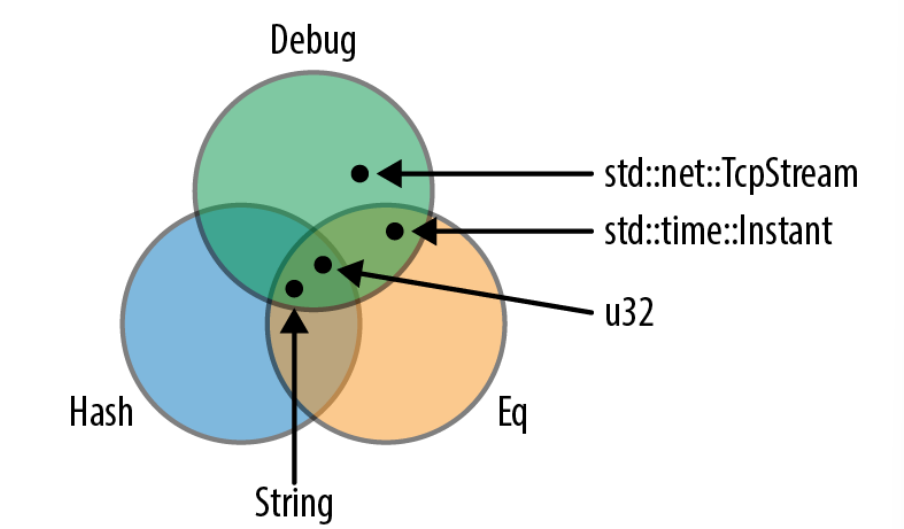
\includegraphics[width=0.8\textwidth]{../img/f11-2.png}
    \caption{trait作为类型的集合}
    \label{f11-2}
\end{figure}

也可以不给类型参数指定任何约束,但这样的话你几乎不能对它进行任何操作。你只能移动它、将它放在box或vector里。

泛型函数可以有多个类型参数:
\begin{minted}{Rust}
    /// 在一个大规模的分区数据集上进行查询。
    /// 见<http://research.google.com/archive/mapreduce.html>。
    fn run_query<M: Mapper + Serialize, R: Reducer + Serialize>(
        data: &DataSet, map: M, reduce: R) -> Results
    { ... }
\end{minted}

正如这个例子展示的一样,约束可能太长以至于很难阅读。Rust提供了使用关键字\texttt{where}的替代语法:
\begin{minted}{Rust}
    fn run_query<M, R>(data: &DataSet, map: M, reduce: R) -> Results
        where M: Mapper + Serialize,
              R: Reducer + Serialize
    { ... }
\end{minted}

类型参数\texttt{M}和\texttt{R}仍然在前边声明,但约束被移动到单独的行。这种\texttt{where}语法可以用于泛型结构体、泛型枚举、类型别名以及方法——任何允许约束的地方。

当然,\texttt{where}语法的一个替代是保持简单:寻找一种不需要大量使用泛型的方法来编写程序。

“\nameref{RefAsArg}”介绍了生命周期的语法。一个泛型函数可以同时有生命周期参数和类型参数。生命周期参数在前:
\begin{minted}{Rust}
    /// 返回`candidates`中距离`target`最近的点的引用。
    fn nearest<'t, 'c, P>(target: &'t P, candidates: &'c [P]) -> &'c P
        where P: MeasureDistance
    {
        ...
    }
\end{minted}

这个函数有两个参数:\texttt{target}和\texttt{candidates}。它们都是引用,但我们给了它们不同的生命周期\texttt{'t}和\texttt{'c}(正如在“\nameref{DistLife}”中讨论的那样)。这个函数可以用于任何实现了\texttt{MeasureDistance} trait的类型\texttt{P},因此我们可以在一个程序中用\texttt{Point2d}值调用它,而在另一个程序中用\texttt{Point3d}值调用它。

生命周期绝不会影响到机器码。两个\texttt{P}的类型相同但生命周期不同的\texttt{nearest()}的调用,将会调用同一个编译好的函数。只有不同的类型才会导致Rust编译一个泛型函数的多个拷贝。

当然,函数并不是Rust中唯一的泛型代码:
\begin{itemize}
    \item 我们已经在“\nameref{GenStruct}”和“\nameref{GenEnum}”中介绍过泛型类型了。
    \item 一个单独的方法也可以是泛型的,就算定义它的类型不是泛型的:
    \begin{minted}{Rust}
    impl PancakeStack {
        fn push<T: Topping>(&mut self, goop: T) -> PancakeResult<()> {
            goop.pour(&self);
            self.absorb_topping(goop)
        }
    }
    \end{minted}
    \item 类型别名也可以是泛型的:
    \begin{minted}{Rust}
    type PancakeResult<T> = Result<T, PancakeError>;
    \end{minted}
    \item 我们将在本章稍后介绍泛型trait。
\end{itemize}

所有这一节中介绍的特性——约束、\texttt{where}子句、生命周期参数等——可以被用于所有泛型item,而不仅仅是函数。

\subsection{选择哪一种}
选择trait对象还是泛型代码是一件很微妙的事情。因为它们都基于trait,有很多相似之处。

任何当你需要一个混合类型的值的集合的情况下trait对象都是正确的选择。从技术上讲创建泛型的沙拉是可行的:
\begin{minted}{Rust}
    trait Vegetable {
        ...
    }

    struct Salad<V: Vegetable> {
        veggies: Vec<V>
    }
\end{minted}

然而,这是一个非常糟糕的设计。每一个这样的沙拉都全部是由单一类型的蔬菜组成的。不是所有人都适合这么做,这本书的作者曾经为一个\texttt{Salad<IcebergLettuce}支付了\$14美元,并且直到现在也没有完全克服那次经历。

然而我们怎么构建一个更好的沙拉呢?因为\texttt{Vegetable}值可能是不同大小的,我们不能要求Rust创建一个\texttt{Vec<dyn Vegetable>}:
\begin{minted}{Rust}
    struct Salad {
        veggies: Vec<dyn Vegetable> // 错误:`dyn Vegetable`并
                                    // 没有固定大小
    }
\end{minted}

trait对象就是解决方案:
\begin{minted}{Rust}
    struct Salad {
        veggies: Vec<Box<dyn Vegetable>>
    }
\end{minted}

每一个\texttt{Box<dyn Vegetable>}可以持有任何类型的蔬菜,但box自身的大小是固定的——两个指针——因此可以存储在vector中。除了在食物里放盒子这个不幸的比喻之外,它确实就是我们需要的。它也同样适用于绘图应用中的形状、游戏中的怪物、网络路由器中的可插拔路由算法等等。

另一个使用trait对象的可能的原因是减小编译出的代码的体积。Rust可能需要编译一个泛型函数很多次,因为它要为每一个用到的类型都编译一次。这可能导致生成的二进制文件很大,这种现象在C++圈子里称为\emph{代码膨胀(code bloat)}。近年来内存越来越充裕,因此我们中的大多数人可以忽略代码的体积,但确实还有一些受限制的环境。

除了涉及到沙拉或者资源受限的环境之外,泛型与trait对象相比有三个优势。因此在Rust中泛型是更加普遍的选择。

第一个优势是速度。注意泛型函数签名中没有\texttt{dyn}关键字。因为你在编译期指明了确切的类型,不管是显式还是通过类型推导,编译器都知道实际上调用了哪个\texttt{write}。没有使用\texttt{dyn}关键字是因为没有trait对象——因此也没有涉及动态分发。

引言中展示的泛型\texttt{min()}函数就和我们单独编写\texttt{min\_u8}、\texttt{min\_i64}、\texttt{min\_string}等函数一样快。编译器还可以像其他函数一样内联它,因此在release构建中,一个对\texttt{min::<i32>}的调用可能只有两三条指令。对于常量的调用,例如\texttt{min(5, 3)}可能会更快:Rust可以在编译期对它进行求值,因此不会有任何运行时开销。

或者考虑这个泛型函数调用:
\begin{minted}{Rust}
    let mut sink = std::io::sink();
    say_hello(&mut sink);
\end{minted}

\texttt{std::io::sink()}返回一个\texttt{Sink}类型的writer,它会偷偷丢弃掉所有写入的字节。

当Rust为此生成机器码的时候,它可以产生先调用\texttt{Sink::write\_all}、再检查错误、最后调用\texttt{Sink::flush}的代码。这正是泛型函数体的内容。

或者,Rust可以查看那些方法,然后意识到下列情况:
\begin{itemize}
    \item \texttt{Sink::write\_all()}什么也不做。
    \item \texttt{Sink:flush()}什么也不做。
    \item 两个方法都不可能返回错误。
\end{itemize}

简单来说,Rust拥有所有优化掉这个函数调用所需的信息。

相比与trait对象的行为,Rust直到运行时才能知道一个trait对象指向的值到底是什么类型。因此即使你传递了一个\texttt{Sink},虚方法的调用开销和检查错误的开销仍然不可避免。

泛型的第二个优势是有的trait不支持trait对象。trait只支持一部分特性,例如关联函数只能使用泛型,这样就完全排除了trait对象。当我们将到这些特性时会指出它们。

泛型的第三个优势是可以很容易地一次给泛型类型参数添加多个trait约束,例如我们的\texttt{top\_ten}函数就要求它的参数\texttt{T}要实现\texttt{Debug + Hash + Eq}。trait对象不能这么做:Rust不支持类似\texttt{\&mut (dyn Debug + Hash + Eq)}这样的类型。(你可以用本章中稍后会讲到的\hyperref[subtrait]{子trait}来实现类似的功能,但这样有点复杂。)

\section{定义和实现trait}

定义一个trait很简单,只需要给出名字和trait方法的签名类型。假设我们在编写一个游戏,我们可能会定义像这样的trait:
\begin{minted}{Rust}
    /// 一个角色、物品、风景等
    /// 任何可以显示在屏幕上的游戏世界的物体。
    trait Visible {
        /// 在给定的画布上渲染这个对象。
        fn draw(&self, canvas: &mut Canvas);

        /// 如果点击(x, y)会选中这个对象就返回true。
        fn hit_test(&self, x: i32, y: i32) -> bool;
    }
\end{minted}

为了实现一个trait,需要使用语法\texttt{impl TraitName for Type}:
\begin{minted}{Rust}
    impl Visible for Broom {
        fn draw(&self, canvas: &mut Canvas) {
            for y in self.y - self.height -1 .. self.y {
                canvas.write_at(self.x, y, '|');
            }
            canvas.write_at(self.x, self.y , 'M);
        }

        fn hit_test(&self, x: i32, y: i32) -> bool {
            self.x == x
            && self.y - self.height - 1 <= y
            && y <= self.y
        }
    }
\end{minted}

注意\texttt{impl}包含了一份\texttt{Visible} trait中每个方法的实现,除此之外没有别的内容。在trait \texttt{impl}中定义的任何东西都必须是trait的特性。如果我们想要添加一个\texttt{Broom::draw()}的帮助函数,我们必须在单独的\texttt{impl}块中定义它:

\begin{minted}{Rust}
    impl Broom {
        /// 下面的Broom::draw()用到的帮助函数。
        fn broomstick_range(&self) -> Range<i32> {
            self.y - self.height - 1 .. self.y
        }
    }
\end{minted}

这些帮助函数可以在trait \texttt{impl}块中使用:
\begin{minted}{Rust}
    impl Visible for Broom {
        fn draw(&self, canvas: &mut Canvas) {
            for y in self.broomstick_range() {
                ...
            }
            ...
        }
        ...
    }
\end{minted}

\subsection{默认方法}
我们之前讨论的\texttt{Sink} writer可以用少数几行代码实现。首先,我们定义如下类型:
\begin{minted}{Rust}
    /// 一个忽略写入数据的writer
    pub struct Sink;
\end{minted}

\texttt{Sink}是一个空结构体,因为我们不需要在里面存储任何数据。接下来,我们为\texttt{Sink}提供了一份\texttt{Write} trait的实现:
\begin{minted}{Rust}
    use std::io::{Write, Result};

    impl Write for Sink {
        fn write(&mut self, buf: &[u8]) -> Result<usize> {
            // 假装成功写入了整个缓冲区
            Ok(buf.len())
        }

        fn flush(&mut self) -> Result<()> {
            Ok(())
        }
    }
\end{minted}

到目前为止,这和\texttt{Visible} trait很像。但是我们展示过\texttt{Write} trait还有一个\texttt{write\_all}方法:
\begin{minted}{Rust}
    let mut out = Sink;
    out.write_all(b"hello world\n")?;
\end{minted}

为什么Rust允许我们\texttt{impl Write for Sink}时不定义\texttt{write\_all}方法?答案就是标准库中\texttt{Write} trait的定义中包含了一个\texttt{write\_all}的\emph{默认实现}:
\begin{minted}{Rust}
    trait Write {
        fn write(&mut self, buf: &[u8]) -> Result<usize>;
        fn flush(&mut self) -> Result<()>;
        
        fn write_all(&mut self, buf: &[8]) -> Result<()> {
            let mut bytes_written = 0;
            while bytes_written < buf.len() {
                bytes_written += self.write(&buf[bytes_written..])?;
            }
            Ok(())            
        }

        ...
    }
\end{minted}

\texttt{write}和\texttt{flush}方法是每一个writer必须实现的基本方法。一个writer可能也实现了\texttt{write\_all},但如果没有,将会使用我们上边展示的默认实现。

你自己的trait也可以使用相同的语法包含默认实现。

默认方法最有戏剧性的使用是在标准库的\texttt{Iterator} trait,它只有一个需要实现的方法\texttt{.next()},和一堆默认实现的方法。\hyperref[ch15]{第15章}中会解释原因。

\subsection{trait和其他人的类型}
Rust允许你在任意类型上实现任意trait,只要trait或者类型是在当前crate中定义的。

这意味着任何时候如果你想给任何类型添加一个方法,你都可以用trait来做到这一点:
\begin{minted}{Rust}
    trait IsEmoji {
        fn is_emoji(&self) -> bool;
    }

    /// 为内建的字符类型实现IsEmoji方法
    impl IsEmoji for char {
        fn is_emoji(&self) -> bool {
            ...
        }
    }

    assert_eq!('$'.is_emoji(), false);
\end{minted}

类似于其他trait方法,只有当\texttt{IsEmoji}在作用域中时新的\texttt{is\_emoji}方法才可见。

这个trait的唯一目的就是给现有类型\texttt{char}添加一个方法。这被称为\emph{扩展trait(extension trait)}。当然,你可以把这个trait添加给其他类型,例如\texttt{impl IsEmoji for str \{ ... \}}等。

你甚至可以使用泛型\texttt{impl}块来一次性给一整个家族的类型添加一个扩展trait。这个trait可以在任何类型上实现:
\begin{minted}{Rust}
    use std::io::{self, Write};

    /// trait for values to which you can send HTML.
    trait WriteHtml {
        fn write_html(&mut self, html: &HtmlDocument) -> io::Result<()>;
    }
\end{minted}

为所有writer实现这个trait,可以为所有Rust writer添加这个方法:
\begin{minted}{Rust}
    /// 你可以向任意std::io writer写入HTML
    impl<W: Write> WriteHtml for W {
        fn write_html(&mut self, html: &HtmlDocument) -> io::Reuslt<()> {
            ...
        }
    }
\end{minted}

\texttt{impl<W: Write> WriteHtml for W}这一行意思是“对于任何实现了\texttt{Write}的类型\texttt{W},这里有一个为\texttt{W}编写的\texttt{WriteHtml}的实现”。

\texttt{serde}库提供了一个很好的例子,它展示了可以在标准类型上实现用户自定义trait这种能力的重要作用。\texttt{serde}是一个序列化库。也就是说,你可以使用它把任何Rust数据结构写入到磁盘,并在稍后加载它们。这个库定义了一个trait \texttt{Serialize},库支持所有实现了这个trait的数据类型。因此在\texttt{serde}的源码中,为\texttt{bool, i8, i16, i32},数组和元组类型等,包括标准数据结构例如\texttt{Vec}和\texttt{HashMap}都实现了\texttt{Serialize} trait。

这样的结果是\texttt{serde}为所有这些类型添加了一个\texttt{.serialize()}方法。它可以像这样使用:
\begin{minted}{Rust}
    use serde::Serialize;
    use serde_json;

    pub fn save_configuration(config: &HashMap<String, String>) 
        -> std::io::Result<()>
    {
        // 创建一个JSON序列化器来把数据写入到文件。
        let writer = File::create(config_filename())?;
        let mut serializer = serde_json::Serializer::new(writer);

        // serde的`.serialize()`方法负责剩余的内容。
        config.serialize(&mut serializer)?;

        Ok(())
    }
\end{minted}

我们之前说过当你实现一个tarit时,trait和类型至少有一个必须是在当前crate中新定义的。这被称为\emph{孤儿规则(orphan rule)}。它帮助确保tarit的实现是唯一的。你的代码不能\texttt{impl Write for u8},因为\texttt{Write}和\texttt{u8}都是在标准库中定义的。如果Rust允许crate这么做,那么不同的crate中可能会有不同的\texttt{u8}类型的\texttt{Write} trait实现。Rust将不知道为一个方法调用选择哪种实现。

(C++也有一个类似的唯一性约束:一次定义规则。在传统的C++风格中,除了最简单的情况之外,编译器并不会强制这一点,如果你打破了这个规则会遇到未定义行为。

\subsection{trait中的\texttt{Self}}


\subsection{子trait}\label{subtrait}

\section{完全限定方法调用}\label{fullymethod}

